
Before C++20, the erase-remove idiom was commonly used to efficiently delete elements from an STL container. This was a little cumbersome, but not a great burden. It was common to use a function like this for the task:

\begin{lstlisting}[style=styleCXX]
template<typename Tc, typename Tv>
void remove_value(Tc & c, const Tv v) {
	auto remove_it = std::remove(c.begin(), c.end(), v);
	c.erase(remove_it, c.end());
}
\end{lstlisting}

The std::remove() function is from the <algorithms> header. std::remove() searches for the specified value and removes it by shifting elements forward from the end of the container. It does not change the size of the container. It returns an iterator past the end of the shifted range. We then call the container's erase() function to delete the remaining elements.

This two-step process is now reduced to one step with the new uniform erasure function:

\begin{lstlisting}[style=styleCXX]
std::erase(c, 5); // same as remove_value() function
\end{lstlisting}

This one function call does the same thing as the remove\_value() function we wrote above.

There's also a version that uses a predicate function. For example, to remove all even numbered values from a numeric container:

\begin{lstlisting}[style=styleCXX]
std::erase_if(c, [](auto x) { return x % 2 == 0; });
\end{lstlisting}

Let's look at the uniform erasure functions in a bit more detail.

\subsubsection{How to do it…}

There are two forms of the uniform erasure functions. The first form, called erase(), takes two parameters, a container and a value:

\begin{lstlisting}[style=styleCXX]
erase(container, value);
\end{lstlisting}

The container may be any of the sequential containers (vector, list, forward\_list, deque), except array, which cannot change size.

The second form, called erase\_if(), takes a container and a predicate function:

\begin{lstlisting}[style=styleCXX]
erase_if(container, predicate);
\end{lstlisting}

This form works with any of the containers that work with erase(), plus the associative containers, set, map, and their multi-key and unordered variants.

The functions erase() and erase\_if() are defined, as non-member functions, in the header for the corresponding container. There is no need to include another header.

Let's look at some examples:

\begin{itemize}
\item 
First, let's define a simple function to print the size and elements of a sequential container:

\begin{lstlisting}[style=styleCXX]
void printc(auto & r) {
	cout << format("size({}) ", r.size());
	for( auto & e : r ) cout << format("{} ", e);
	cout << "\n";
}
\end{lstlisting}

The printc() function uses the C++20 format() function to format a string for cout.

\item 
Here's a vector with 10 integer elements, printed with our printc() function:

\begin{lstlisting}[style=styleCXX]
vector v{ 1, 2, 3, 4, 5, 6, 7, 8, 9 };
printc(v);
\end{lstlisting}

Output:

\begin{tcblisting}{commandshell={}}
size: 10: 0 1 2 3 4 5 6 7 8 9
\end{tcblisting}

We see that the vector has 10 elements. Now we can use erase() to remove all elements with the value 5:

\begin{lstlisting}[style=styleCXX]
erase(v, 5);
printc(v);
\end{lstlisting}

Output:

\begin{tcblisting}{commandshell={}}
size: 9: 0 1 2 3 4 6 7 8 9
\end{tcblisting}

The vector version of the std::erase() function is defined in the <vector> header. After the erase() call, the element with the value 5 has been removed and the vector has 9 elements.

\item 
This works just as well with a list container:

\begin{lstlisting}[style=styleCXX]
list l{ 0, 1, 2, 3, 4, 5, 6, 7, 8, 9 };
printc(l);
erase(l, 5);
printc(l);
\end{lstlisting}

Output:

\begin{tcblisting}{commandshell={}}
size: 10: 0 1 2 3 4 5 6 7 8 9
size: 9: 0 1 2 3 4 6 7 8 9
\end{tcblisting}

The list version of the std::erase() function is defined in the <list> header. After the erase() call, the element with the value 5 has been removed and the list has 9 elements.

\item 
We can use erase\_if() to remove all the even numbered elements with a simple predicate function:

\begin{lstlisting}[style=styleCXX]
vector v{ 0, 1, 2, 3, 4, 5, 6, 7, 8, 9 };
printc(v);
erase_if(v, [](auto x) { return x % 2 == 0; });
printc(v);
\end{lstlisting}

Output:

\begin{tcblisting}{commandshell={}}
size: 10: 0 1 2 3 4 5 6 7 8 9
size: 5: 1 3 5 7 9
\end{tcblisting}

\item 
The erase\_if() function also works with associative containers, like map:

\begin{lstlisting}[style=styleCXX]
void print_assoc(auto& r) {
	cout << format("size: {}: ", r.size());
	for( auto& [k, v] : r ) cout << format("{}:{} ",
		k, v);
	cout << "\n";
}

int main() {
	map<int, string> m{ {1, "uno"}, {2, "dos"},
		{3, "tres"}, {4, "quatro"}, {5, "cinco"} };
	print_assoc(m);
	erase_if(m,
		[](auto& p) { auto& [k, v] = p;
		return k % 2 == 0; }
	);
	print_assoc(m);
}
\end{lstlisting}

Output:

\begin{tcblisting}{commandshell={}}
size: 5: 1:uno 2:dos 3:tres 4:quatro 5:cinco
size: 3: 1:uno 3:tres 5:cinco
\end{tcblisting}

Because each element of a map is returned as a pair, we need a different function to print them. The print\_assoc() function unpacks the pair elements with a structured binding in the for loop. We also use a structured binding in the predicate function of erase\_if() to isolate the key for filtering the even numbered elements.
\end{itemize}

\subsubsection{How it works…}

The erase() and erase\_if() functions are simply wrappers that perform the eraseremove idiom in one step. They perform the same operations as a function, like this:

\begin{lstlisting}[style=styleCXX]
template<typename Tc, typename Tv>
void remove_value(Tc & c, const Tv v) {
	auto remove_it = std::remove(c.begin(), c.end(), v);
	c.erase(remove_it, c.end());
}
\end{lstlisting}

If we consider a simple vector of int, called vec, with the following values:

\begin{lstlisting}[style=styleCXX]
vector vec{ 0, 1, 2, 3, 4, 5, 6, 7, 8, 9 };
\end{lstlisting}

We can visualize vec as a one-row table of int values:

\hspace*{\fill} \\ %插入空行
\begin{center}
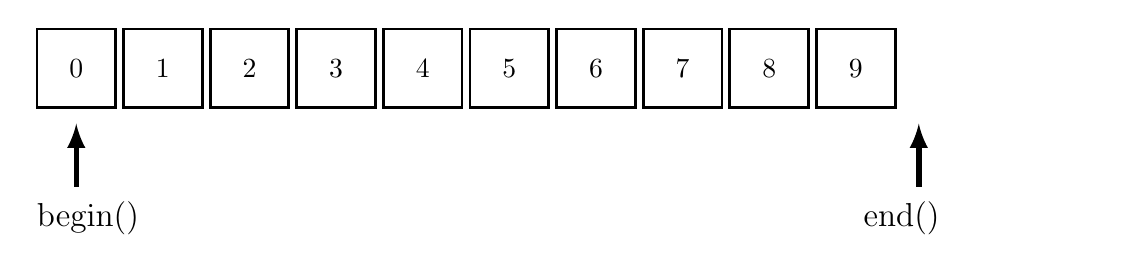
\begin{tikzpicture}
\foreach \x in {0,...,9} {
	\draw[line width=1pt] (1.1*\x,1) rectangle (1.1*\x+1,0) node[pos=.5] {\x};
}

\draw[line width=2pt][-latex] (0.5,-1.0) -- (0.5,-0.2);
\draw[line width=2pt][-latex] (11.2,-1.0) -- (11.2,-0.2);

\node[text width=3cm, font=\large] at (1.5,-1.4) {begin()};
\node[text width=3cm, font=\large] at (12,-1.4) {end()};
\end{tikzpicture}

Figure 3.1 – begin() and end() iterators
\end{center}

The begin() iterator points at the first element, and the end() iterator points past the last element. This configuration is standard for all STL sequential containers.

When we call remove(c.begin(), c.end(), 5), the algorithm searches for matching elements, starting at the begin() iterator. For each matching element that it finds, it shifts the next element into its place. It continues searching and shifting until it reaches the end() iterator. The result is a container where all the remaining elements are at the beginning, without the deleted elements, and in their original order. The end() iterator is unchanged and the remaining elements are undefined. We can visualize the operation like this:

\hspace*{\fill} \\ %插入空行
\begin{center}
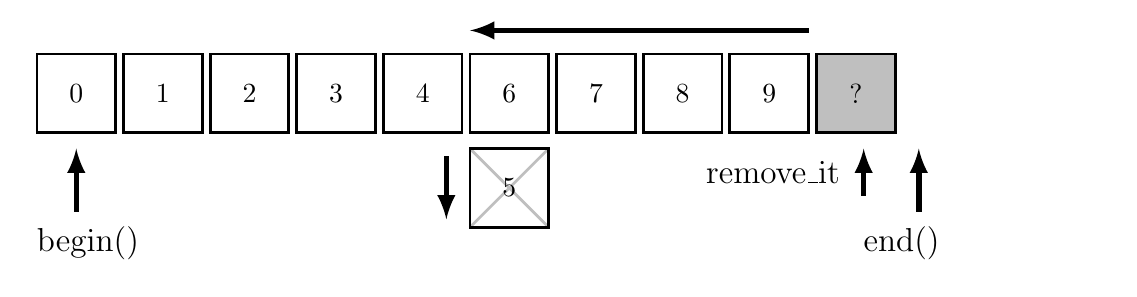
\begin{tikzpicture}
\draw[line width=2pt][-latex] (9.8,1.3) -- (5.5,1.3);
	
\foreach \x in {0,...,4} {
	\draw[line width=1pt] (1.1*\x,1) rectangle (1.1*\x+1,0) node[pos=.5] {\x};
}

\foreach \x [evaluate=\x as \index using int(\x+1)] in {5,...,9} {
	\draw[line width=1pt] (1.1*\x,1) rectangle (1.1*\x+1,0) node[pos=.5] {\index};
}

\foreach \x in {9} {
	\draw[fill=white!50!gray, line width=1pt] (1.1*\x,1) rectangle (1.1*\x+1,0) node[pos=.5] {?};
}

\draw[line width=2pt][-latex] (0.5,-1.0) -- (0.5,-0.2);
\draw[line width=2pt][-latex] (11.2,-1.0) -- (11.2,-0.2);
\draw[line width=2pt][-latex] (5.2,-0.3) -- (5.2,-1.1);
\draw[line width=2pt][-latex] (10.5,-0.8) -- (10.5,-0.2);

\draw[color=white!50!gray, line width=1pt] (1.1*5,-0.2) -- (1.1*5+1,-1.2); 
\draw[color=white!50!gray, line width=1pt] (1.1*5,-1.2) -- (1.1*5+1,-0.2);
\draw[line width=1pt] (1.1*5,-0.2) rectangle (1.1*5+1,-1.2) node[pos=.5] {5};

\node[text width=3cm, font=\large] at (1.5,-1.4) {begin()};
\node[text width=3cm, font=\large] at (12,-1.4) {end()};
\node[text width=3cm, font=\large] at (10.0,-0.5) {remove\_it};
\end{tikzpicture}

Figure 3.2 – Removing an element
\end{center}

The remove() function returns an iterator (remove\_it) that points to the first element past the elements that were shifted. The end() iterator remains as it was before the remove() operation. To further illustrate, if we were to remove all even-numbered elements using remove\_if(), our result would look like this:

\hspace*{\fill} \\ %插入空行
\begin{center}
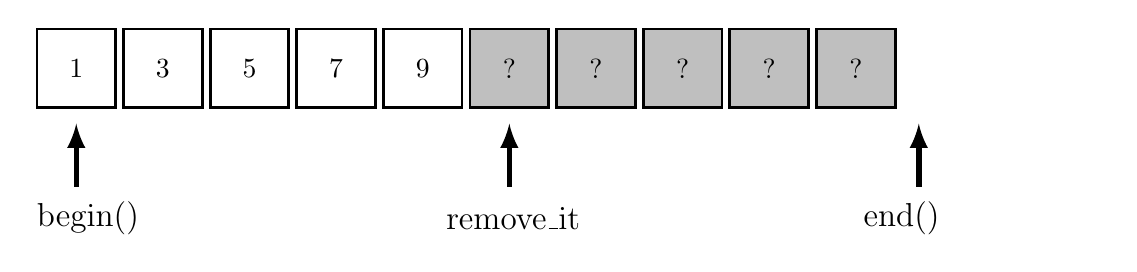
\begin{tikzpicture}

\foreach \x [evaluate=\x as \index using int(2*\x+1)] in {0,...,4} {
	\draw[line width=1pt] (1.1*\x,1) rectangle (1.1*\x+1,0) node[pos=.5] {\index};
}

\foreach \x [evaluate=\x as \index using int(\x+1)] in {5,...,9} {
	\draw[fill=white!50!gray, line width=1pt] (1.1*\x,1) rectangle (1.1*\x+1,0) node[pos=.5] {?};
}

\draw[line width=2pt][-latex] (0.5,-1.0) -- (0.5,-0.2);
\draw[line width=2pt][-latex] (6.0,-1.0) -- (6.0,-0.2);
\draw[line width=2pt][-latex] (11.2,-1.0) -- (11.2,-0.2);

\node[text width=3cm, font=\large] at (1.5,-1.4) {begin()};
\node[text width=3cm, font=\large] at (6.7,-1.4) {remove\_it};
\node[text width=3cm, font=\large] at (12,-1.4) {end()};
\end{tikzpicture}
	
Figure 3.3 – After removing even-numbered elements
\end{center}

In this case, all that remains is the five odd-numbered elements followed by five elements of undefined value.

The container's erase() function is then called to erase the remaining elements:

\begin{lstlisting}[style=styleCXX]
c.erase(remove_it, c.end());
\end{lstlisting}

The container's erase() function is called with the remove\_it and end() iterators to delete all the undefined elements.

The erase() and erase\_if() functions call both the remove() function and the container's erase() function, in order to perform the erase-remove idiom in one step.




